\chapter{Evaluation and Discussion}
\label{chap:eval}

This chapter reports the outcomes of the three experimental contrasts of Chapter~\ref{chap:methodology} on the held-out test subset of the dataset. Section~\ref{sec:results_protocol} describes how the runs are selected and how the acceptance bounds are interpreted. Section~\ref{sec:results_capacity} discusses the first contrast (generator capacity). Section~\ref{sec:results_adversarial} discusses the second contrast (regression versus adversarial fine-tune). Section~\ref{sec:results_conditioning} discusses the third contrast (conditioning on the scalar vector). Section~\ref{sec:results_summary} closes with a synthesis across the three contrasts and outlines the limitations.


\subsection{Regression Stage}
\label{subsec:results_regression}

\begin{figure}[t]
\centering
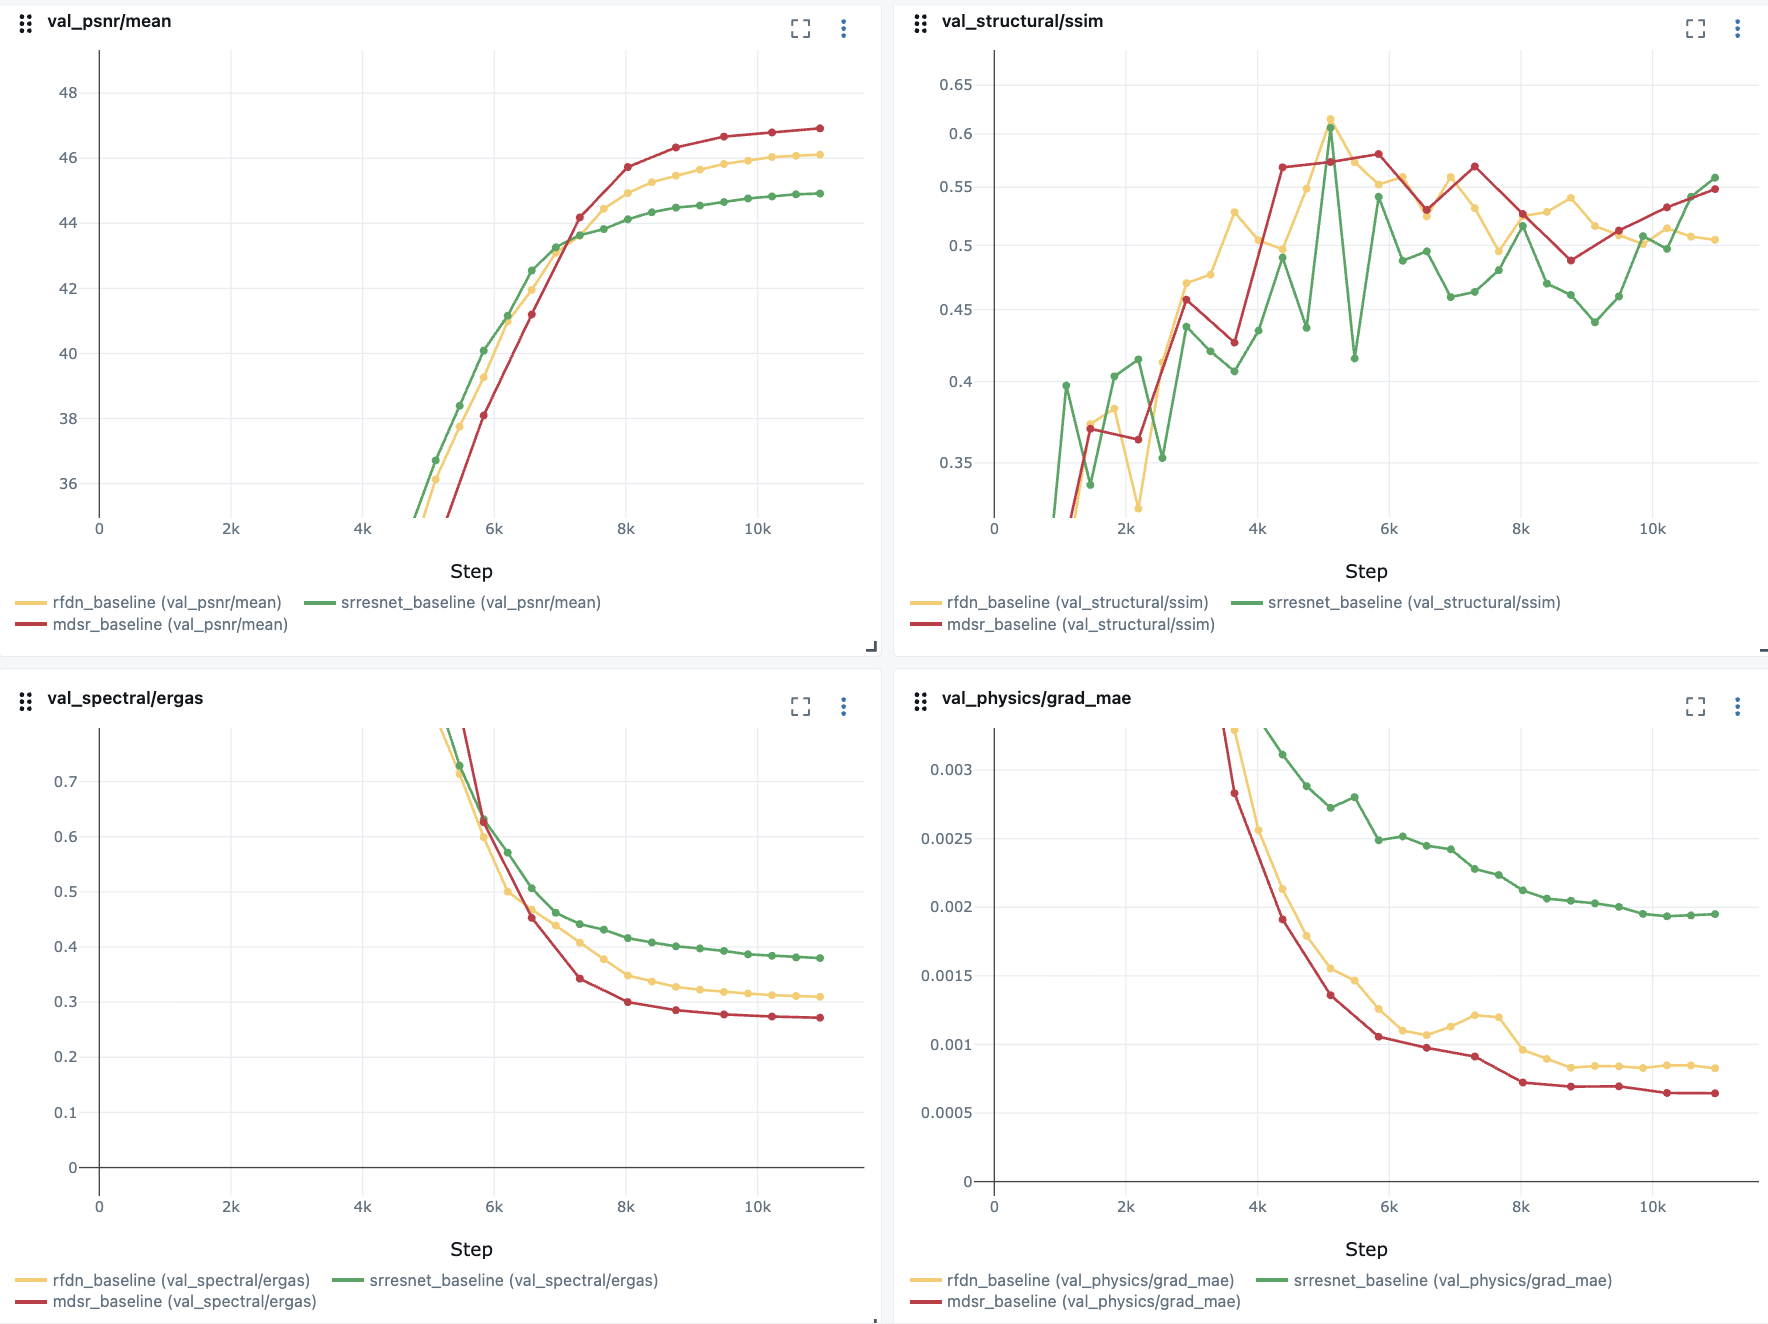
\includegraphics[width=\textwidth]{figures/val_psnr_ssim_ergas_gmae_generators.png}
\caption{Validation metrics over training epochs for the three generators in the regression stage.}
\label{fig:val_generators}
\end{figure}

EDSR (recorded in the logs under the label MDSR) follows the smoothest of the three trajectories. The pixel loss falls from $0.08$ at the start of training to $1.3 \cdot 10^{-3}$ at the end of one hundred fifty epochs, with the gradient norm decaying from approximately $2$ to $0.5$ over the same horizon and no instability in between. The PSNR climbs from $7$ dB at the tenth validation pass through the thirty-decibel threshold around epoch sixty to a final plateau near $46.8$ dB; the channel-wise breakdown at the last epoch puts the pressure channel at $43.5$ dB and the two saturation channels at $51.4$ and $51.8$ dB, consistent with the wider dynamic range of pressure. SSIM behaves differently: it rises to a peak of $0.63$ near epoch eighty, drifts down to $0.44$ by epoch one hundred thirty, and recovers only partially to $0.55$ at the end. The drift away from the SSIM peak coincides with the second half of the regression schedule, where the pixel loss continues to fall but the structure of the displacement fronts begins to smooth out under the unrestrained $L_1$ objective.

MSRResNet converges more slowly and to a lower ceiling. The first five validation passes leave the network essentially untrained, with the validation loss still near $0.8$ and PSNR around one decibel, against the seven decibels reached by the deeper network at the same milestone. From epoch ten onward the trajectory normalizes, the training loss settles into the same $0.08 \to 1.4 \cdot 10^{-3}$ band, and the gradient norm contracts from $2.0$ to $0.15$. Final PSNR reaches $44.94$ dB and the channel split is $42.2$ / $46.9$ / $49.1$ dB for $P$, $S$, and $\bar{S}$, with the pressure channel trailing the saturations as in the larger backbone. SSIM shows the same regression-stage instability, swinging between $0.42$ and $0.61$ over neighboring validation passes around epoch seventy and finishing at $0.56$ after a long plateau in which PSNR adds barely more than two decibels across fifty epochs, signaling that the capacity of the network has been reached.

RFDN occupies an intermediate position despite the smallest parameter count. Its training loss follows the curve $0.09 \to 1.1 \cdot 10^{-3}$ with a gradient norm that contracts from $1.6$ to $0.07$, the cleanest of the three. PSNR starts slowly, sits at $4.6$ dB by epoch four, and converges by the tenth epoch to a trajectory that ends at $46.11$ dB at the final checkpoint, $1.2$ dB above MSRResNet and $0.7$ dB below EDSR at a fraction of the parameter budget. The channel breakdown $43.1$ / $49.5$ / $51.1$ dB for $P$, $S$, and $\bar{S}$ tracks EDSR closely, which suggests that the spatial attention block compensates for the narrower feature width on the saturation channels. SSIM peaks at $0.61$ around epoch seventy and drifts down to $0.50$ at the final checkpoint, repeating the structural-quality drop seen on the other two trajectories.

Figure~\ref{fig:val_generators} overlays the three runs on common axes for PSNR, SSIM, ERGAS, and GMAE. The shared pattern is a decoupling between the pixel objective and the structural metric in the second half of the schedule: PSNR continues to rise, the pixel loss continues to fall, and SSIM moves in the opposite direction by between $0.06$ and $0.11$ points relative to its peak. The peak SSIM is reached on every backbone around epoch seventy to eighty, well before the final checkpoint, and is the natural reference point for the warm start of the adversarial stage.


\subsection{Adversarial Stage}
\label{subsec:results_adversarial}

\begin{figure}[t]
\centering
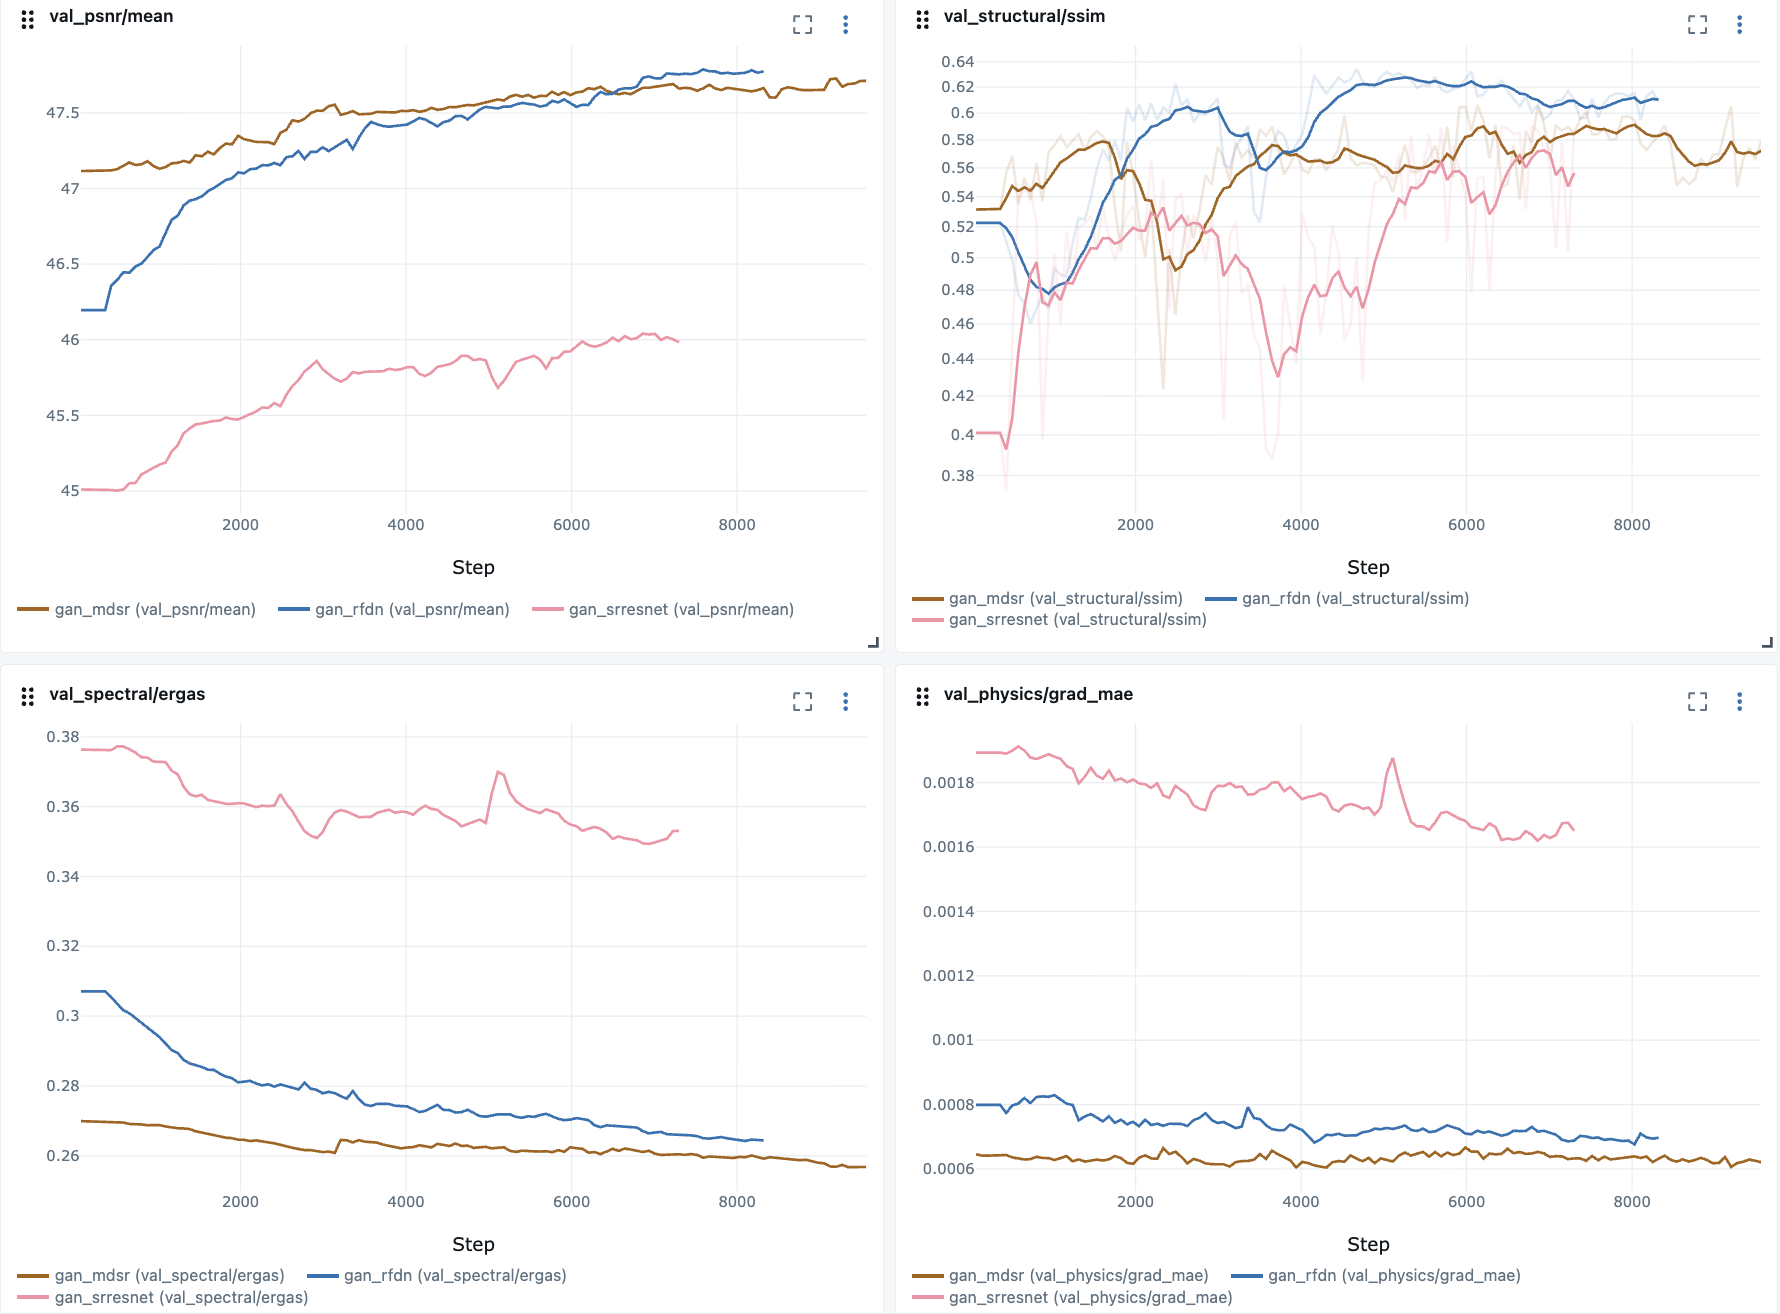
\includegraphics[width=\textwidth]{figures/val_psnr_ssim_ergas_gmae_gans.png}
\caption{Validation metrics over training epochs for the three generators in the adversarial stage.}
\label{fig:val_gans}
\end{figure}

EDSR follows the cleanest of the three adversarial trajectories. The five-epoch discriminator warmup settles its loss near $\ln 2 \approx 0.69$, the five-epoch generator warmup on the pixel and perceptual terms raises SSIM from $0.53$ to $0.57$ without touching PSNR, and the full composite objective then opens with a textbook relativistic equilibrium: the critic-to-generator loss ratio sits at one and the logit gap at zero for nine epochs. From epoch nineteen onward the discriminator starts to separate real residuals from fakes, the logit gap grows to $0.05$, and the adversarial term begins to deliver gradient. The structural score reaches a first local peak of $0.60$ at epoch forty-one and a global peak of $0.61$ at epoch ninety-three; PSNR climbs to $47.71$ dB at epoch one hundred thirty and the channel split at that point is $44.3$ / $53.5$ / $52.3$ dB for $P$, $S$, and $\bar{S}$. From epoch fifty-six the skip rule starts to fire whenever the critic becomes too confident on the current batch, which keeps it from overwhelming the generator and explains the absence of any sign of mode collapse over the full one hundred thirty epochs.

MSRResNet yields the largest relative SSIM gain together with the most volatile training dynamics. The warmup phases follow the same recipe and lift SSIM from $0.40$ to $0.54$ on the perceptual term alone before the discriminator gradient is enabled. The full composite objective then drives the critic into a sequence of swings: at epoch thirty-three its loss briefly rises to $0.77$, then collapses to $\ln 2$ for one validation window before recovering; at epoch sixty-eight the critic-to-generator ratio peaks at $1.54$ and the skip rule activates for two consecutive epochs; from epoch ninety-three onward the rule fires intermittently as the discriminator keeps tightening on the smaller generator. PSNR rises to $46.04$ dB at epoch ninety-three and stabilizes at $45.99$--$46.04$ dB afterwards; SSIM oscillates with an amplitude of about $\pm 0.10$ between epochs but reaches a peak of $0.59$ at epochs eighty-seven, ninety-two, and ninety-five. The final channel split is $43.4$ / $48.3$ / $50.0$ dB for $P$, $S$, and $\bar{S}$, with the pressure channel improving by one decibel relative to the pixel-only baseline.

RFDN gives the most stable trajectory of the three and reaches the highest scores. The skip rule never activates over one hundred thirteen epochs, the critic-to-generator ratio stays in a narrow band around one outside a single excursion to $1.63$ at epoch forty-five, and both networks recover from that excursion without leaving any trace on the generator output. SSIM transiently dips from $0.52$ to $0.46$ during the generator warmup as the perceptual term reshapes the structural content, returns to the baseline by epoch eighteen, and then climbs to a peak of $0.629$ at epoch fifty-six with further peaks above $0.62$ at epochs sixty and sixty-one. PSNR rises steadily to $47.77$ dB at the end of training, the highest of the three adversarial runs, and the channel split $44.6$ / $51.8$ / $52.8$ dB is the most balanced as well, with the pressure channel landing $1.5$ dB above the corresponding pixel-only run.

Figure~\ref{fig:val_gans} places the three runs on common axes for PSNR, SSIM, ERGAS, and GMAE. The shared pattern across the three trajectories is that the warmup decouples the pixel and the perceptual updates, the full composite objective then activates without an early SSIM collapse, and the skip rule contains the discriminator when it becomes overconfident on the current batch. PSNR rises by between one and one and a half decibels relative to the pixel-only baseline on every backbone, SSIM rises by between $0.07$ and $0.13$ points, and no run shows the trade-off between point-wise and structural quality reported in classical SRGAN training.


\section{Summary}
\label{sec:results_summary}

Table~\ref{tab:val_metrics} brings together the validation scores of the six runs against the recalibrated acceptance bounds of the evaluation protocol. A run is counted as accepted when all five scores meet their bounds simultaneously. None of the three pixel-only runs passes the full suite. MSRResNet sits $0.08$ dB below on PSNR, EDSR falls $0.002$ short on SSIM, and RFDN falls $0.045$ below on the same metric. The point-wise scores in the regression stage are otherwise comfortable on all three backbones: GMAE stays between three and thirty times under its bound, ERGAS between one and two orders of magnitude under, and max\_ae is met by EDSR alone. The picture is consistent with the regression-stage trajectories analyzed earlier in this chapter: the pixel objective alone drives PSNR well past the required level on the two deeper backbones but cannot lift SSIM to that level on the displacement fronts.

\begin{table}[t]
\centering
\caption{Validation metrics of the six selected runs against recalibrated acceptance bounds.}
\label{tab:val_metrics}
\small
\setlength{\tabcolsep}{6pt}
\begin{tabular}{l ccccc}
\toprule
Configuration
  & PSNR$\uparrow$ & SSIM$\uparrow$ & GMAE$\downarrow$ & ERGAS$\downarrow$ & max\_ae$\downarrow$ \\
Acceptance bound
  & $\geq 45$ & $\geq 0.55$ & $\leq 0.002$ & $\leq 0.4$ & $\leq 1.5$ \\
\midrule
\multicolumn{6}{l}{Regression stage} \\
\midrule
MSRResNet & 44.92          & \textbf{0.559} & \textbf{0.00195} & \textbf{0.380} & 1.620          \\
EDSR      & \textbf{46.92} & 0.548          & \textbf{0.00064} & \textbf{0.272} & \textbf{1.304} \\
RFDN      & \textbf{46.11} & 0.505          & \textbf{0.00083} & \textbf{0.310} & 1.593          \\
\midrule
\multicolumn{6}{l}{Adversarial fine-tune} \\
\midrule
MSRResNet GAN & \textbf{45.99} & \textbf{0.590} & \textbf{0.00165} & \textbf{0.353} & \textbf{1.380} \\
EDSR GAN      & \textbf{47.71} & \textbf{0.606} & \textbf{0.00062} & \textbf{0.257} & \textbf{1.099} \\
RFDN GAN      & \textbf{47.77} & \textbf{0.634} & \textbf{0.00070} & \textbf{0.264} & \textbf{1.097} \\
\bottomrule
\end{tabular}
\end{table}

The adversarial fine-tune closes the gap on every architecture. All three GAN runs pass all five bounds, with margins between $0.04$ and $0.08$ on SSIM, between $1.0$ and $2.8$ dB on PSNR, and between $0.4$ and $0.5$ on max\_ae. The relative SSIM gain over the corresponding pixel-only run is largest for RFDN ($+0.129$ from $0.505$), which goes from the only backbone that misses three bounds to the configuration with the highest score on every metric in the suite. PSNR rises by between $1.0$ and $1.7$ dB across the three runs, against the conventional trade-off reported for classical adversarial super-resolution in which PSNR is sacrificed for perceptual quality. The composite objective with the dual-porosity physics priors and the discriminator skip rule preserves the point-wise accuracy reached during pixel-only training and adds the structural gain on top.

Model sizes are collected in Table~\ref{tab:model_sizes}. Parameter counts span a factor of two across the three architectures, from $0.79$ million for RFDN to $1.52$ million for EDSR. The PyTorch checkpoint of an adversarial run is roughly four to five times heavier than the regression-stage checkpoint of the same architecture, because the file on disk there carries the discriminator and the moving-average copy of the generator in addition to the generator itself. The exported ONNX artifact, in contrast, contains only the moving-average generator weights, so its size scales with the architecture alone and does not change between the two training stages. ONNX artifacts range from $3.07$ MB for RFDN to $5.81$ MB for EDSR; the larger PyTorch files belong to the development workflow and are not deployed.

\begin{table}[t]
\centering
\caption{Parameter count of the generator and on-disk size of the regression checkpoint, the adversarial checkpoint, and the exported ONNX artifact for the three architectures.}
\label{tab:model_sizes}
\small
\setlength{\tabcolsep}{8pt}
\begin{tabular}{l c c c c}
\toprule
Architecture & Params (M) & Regression ckpt (MB) & Adversarial ckpt (MB) & ONNX (MB) \\
\midrule
RFDN      & 0.79 & 12.31 & 65.66 & 3.07 \\
MSRResNet & 0.93 & 14.22 & 67.53 & 3.55 \\
EDSR      & 1.52 & 23.29 & 76.61 & 5.81 \\
\bottomrule
\end{tabular}
\end{table}

RFDN GAN combines the smallest exported footprint with the highest score on every metric in the quality suite. EDSR GAN places second on PSNR and on max\_ae but trails RFDN GAN on SSIM by $0.028$ points at almost twice the parameter count. MSRResNet GAN passes every bound and is the lightest backbone among those that fail in the pixel-only regime, which makes it the natural candidate for resource-constrained deployment if RFDN is not available.